% !TeX encoding = UTF-8
% !TeX spellcheck = en_US
% !TeX root = main.tex

\documentclass[12pt,a4paper]{memoir}
\usepackage[utf8]{inputenc}
\usepackage{amsmath}
\usepackage{amsfonts}
\usepackage{amssymb}
\usepackage{graphicx}
\usepackage{rotating}
\usepackage{epstopdf}
\usepackage{hyperref}
%\usepackage{indentfirst}
\usepackage[english]{babel}
\usepackage{empheq}

\usepackage[colorinlistoftodos,textsize=scriptsize]{todonotes}

% Default fixed font does  support bold face

% Custom colors
\usepackage{color}
\definecolor{deepblue}{rgb}{0,0,0.5}
\definecolor{deepred}{rgb}{0.6,0,0}
\definecolor{deepgreen}{rgb}{0,0.5,0}
\definecolor{gray}{rgb}{0.5,0.5,0.4}

\usepackage{listings}
\usepackage{lstautogobble}
\renewcommand{\lstlistingname}{Code example}

% Python style for highlighting
\newcommand\pythonstyle{\lstset{
    language=Python,
    basicstyle=\linespread{1}\footnotesize\ttfamily,
    otherkeywords={self},             % Add keywords here
    keywordstyle=\footnotesize\ttfamily\bfseries\color{deepblue},
    emph={MyClass,__init__},          % Custom highlighting
    emphstyle=\bf\color{deepred},    % Custom highlighting style
    stringstyle=\color{deepgreen},
    frame=tb,                         % Any extra options here
    showstringspaces=false,           % 
    tabsize=4,
    numbers=left,    
    numberstyle=\tiny\color{gray}, 
    breaklines=true,
    autogobble=true,
    commentstyle=\color{gray},           
}}


% Python environment
\lstnewenvironment{python}[1][]
{
\pythonstyle
\lstset{#1}
}
{}

% Python for external files
\newcommand\pythonexternal[2][]{{
\pythonstyle
\lstinputlisting[#1]{#2}}}

\newcommand\cppstyle{\lstset{
    language=C++,
    basicstyle=\ttfamily,
    keywordstyle=\color{deepblue}\ttfamily,
    stringstyle=\color{red}\ttfamily,
    commentstyle=\color{grey}\ttfamily,
    morecomment=[l][\color{magenta}]{\#},
    autogobble=true,
}}

% C++ environment
\lstnewenvironment{c++}[1][]
{
    \cppstyle
    \lstset{#1}
}
{}

% % % % % % % % % % % % % % % % % %
% trick not to release comments   %
  \newif\ifrelease
%	                              %
	%\releasetrue
	\releasefalse
%	                              %
	\ifrelease
		\renewcommand{\todo}[1]{}
	\fi
% end of trick                    %
% % % % % % % % % % % % % % % % % %

\renewcommand{\vec}[1]{\underline{#1}}
\newcommand{\mat}[1]{\underline{\underline{#1}}}
\newcommand{\scal}[2]{\langle #1 {\,,\,} #2 \rangle}

\newcommand{\remark}{\paragraph{Remark ---}}
\renewcommand{\epsilon}{\varepsilon}
\setsecnumdepth{subsection}
%\maxtocdepth{subsection}

\def\thetitle{Localisation and correction of orbit perturbations in BESSY II storage ring}
\def\thesubject{Master Thesis}
\def\theauthor{Olivier Churlaud}
\author{\theauthor}
\title{\thetitle}

\hypersetup{
    unicode=true,
    pdftitle={\thetitle},
    pdfauthor={\theauthor},
    pdfsubject={\thesubject},
    colorlinks=true,       % false: boxed links; true: colored links
    linkcolor=black,       % color of internal links (change box color with linkbordercolor)
    citecolor=green,
    filecolor=red,
    urlcolor=blue
}

\begin{document}
\frontmatter
\clearpage
\thispagestyle{empty}
\maketitle
\
\vfill
\begin{abstract}
       ......
\end{abstract}
\vfill

\cleardoublepage

\tableofcontents
\listoffigures

\mainmatter
% !TeX spellcheck = en_US

\chapter{Background and theory}
\label{sec:background}

\section{BESSY II}

\subsection{General presentation}
BESSY II (\textbf{B}erliner \textbf{E}lektronen\-\textbf{S}peicherring-Gesellschaft für \textbf{Sy}n\-chro\-tron\-strahlung m.b.H.) is Berlin electron storage ring, aimed at producing high energy light ray by synchrotron radiation. It emits extremely brillant photons pulse ranging from the long wave terahertz region to hard X rays, with an emphasis on the soft X-ray range~\cite{web:bessy_homepage}. Scientific projects can freely apply to an experimental station, where they are able to adjust the wavelength, polarization and photon energy. More than 2000 scientists per year are using BESSY II equipment.

The storage ring has a circumference of 240~meters and provides around 50 beamlines (paths of light rays between the accelerator and experimental stations). The electrons are accelerated to an energy up to 1.7~GeV.

BESSY II was inaugurated in 1998 and is since 2009 a facility of the \textit{Helmholtz-Zentrum Berlin für Materialien und Energie} (HZB), to study material structures and processes by guest scientists.

Additionally to the guest scientists, experts and operators\todo{I don't know how to call them} ensure the good functioning of the whole facility and work on refining the quality and the stability of the light rays. 

\subsection{General functioning}
The way BESSY II functions is based on the synchrotron radiation phenomenon: any accelerated particle emits radiations (in the form of photons), with a maximal amplitude in the case of a circular acceleration. \todo{Should I detail the equations?} It can be shown~\cite{book:wille} that the radiated power in circular acceleration can be given as 
\begin{equation}
P_s = \frac{e^2 c}{6 \pi \epsilon_0}\frac{1}{(m_0 c^2)^4}\frac{E^4}{R^2}.
\end{equation}
where $c$ is the speed of light, $m_0$ the rest mass (independent of the velocity) of the particle, $e$ its charge, $E$ it's energy, $R$ the bending radius and $\epsilon_0$ the  vacuum permittivity.

Considering their low mass, the electrons are very good candidates to produce high energy radiation.

The most important properties of the synchrotron radiation are its brilliance and brightness, which describe the quality of the beam. The brightness describes the angular divergence of the beam, and the brillance its transverse dimension: both are expected to be as small as possible to be in the configuration in which the beam is the most point-like. (See Section~\ref{sec:brightness_brillance} for the exact definitions).

The main purpose of BESSY II is to provide a light radiation with stable brilliance and brightness over time. To achieve this, the light source itself must be very stable as well. Therefore a significant attention is drawn to the control of the storage ring.
\begin{figure}
	\centering
	\includegraphics[width=0.8\textwidth]{img/bessy_acc_chain_web.jpg}
	\caption[Bessy II -- Accelerator chain]{\label{fig:bessy_acc_web_simple} Bessy II -- Accelerator chain (Source:~\cite{web:bessy_homepage})}
\end{figure}

\begin{sidewaysfigure}
    \centering
    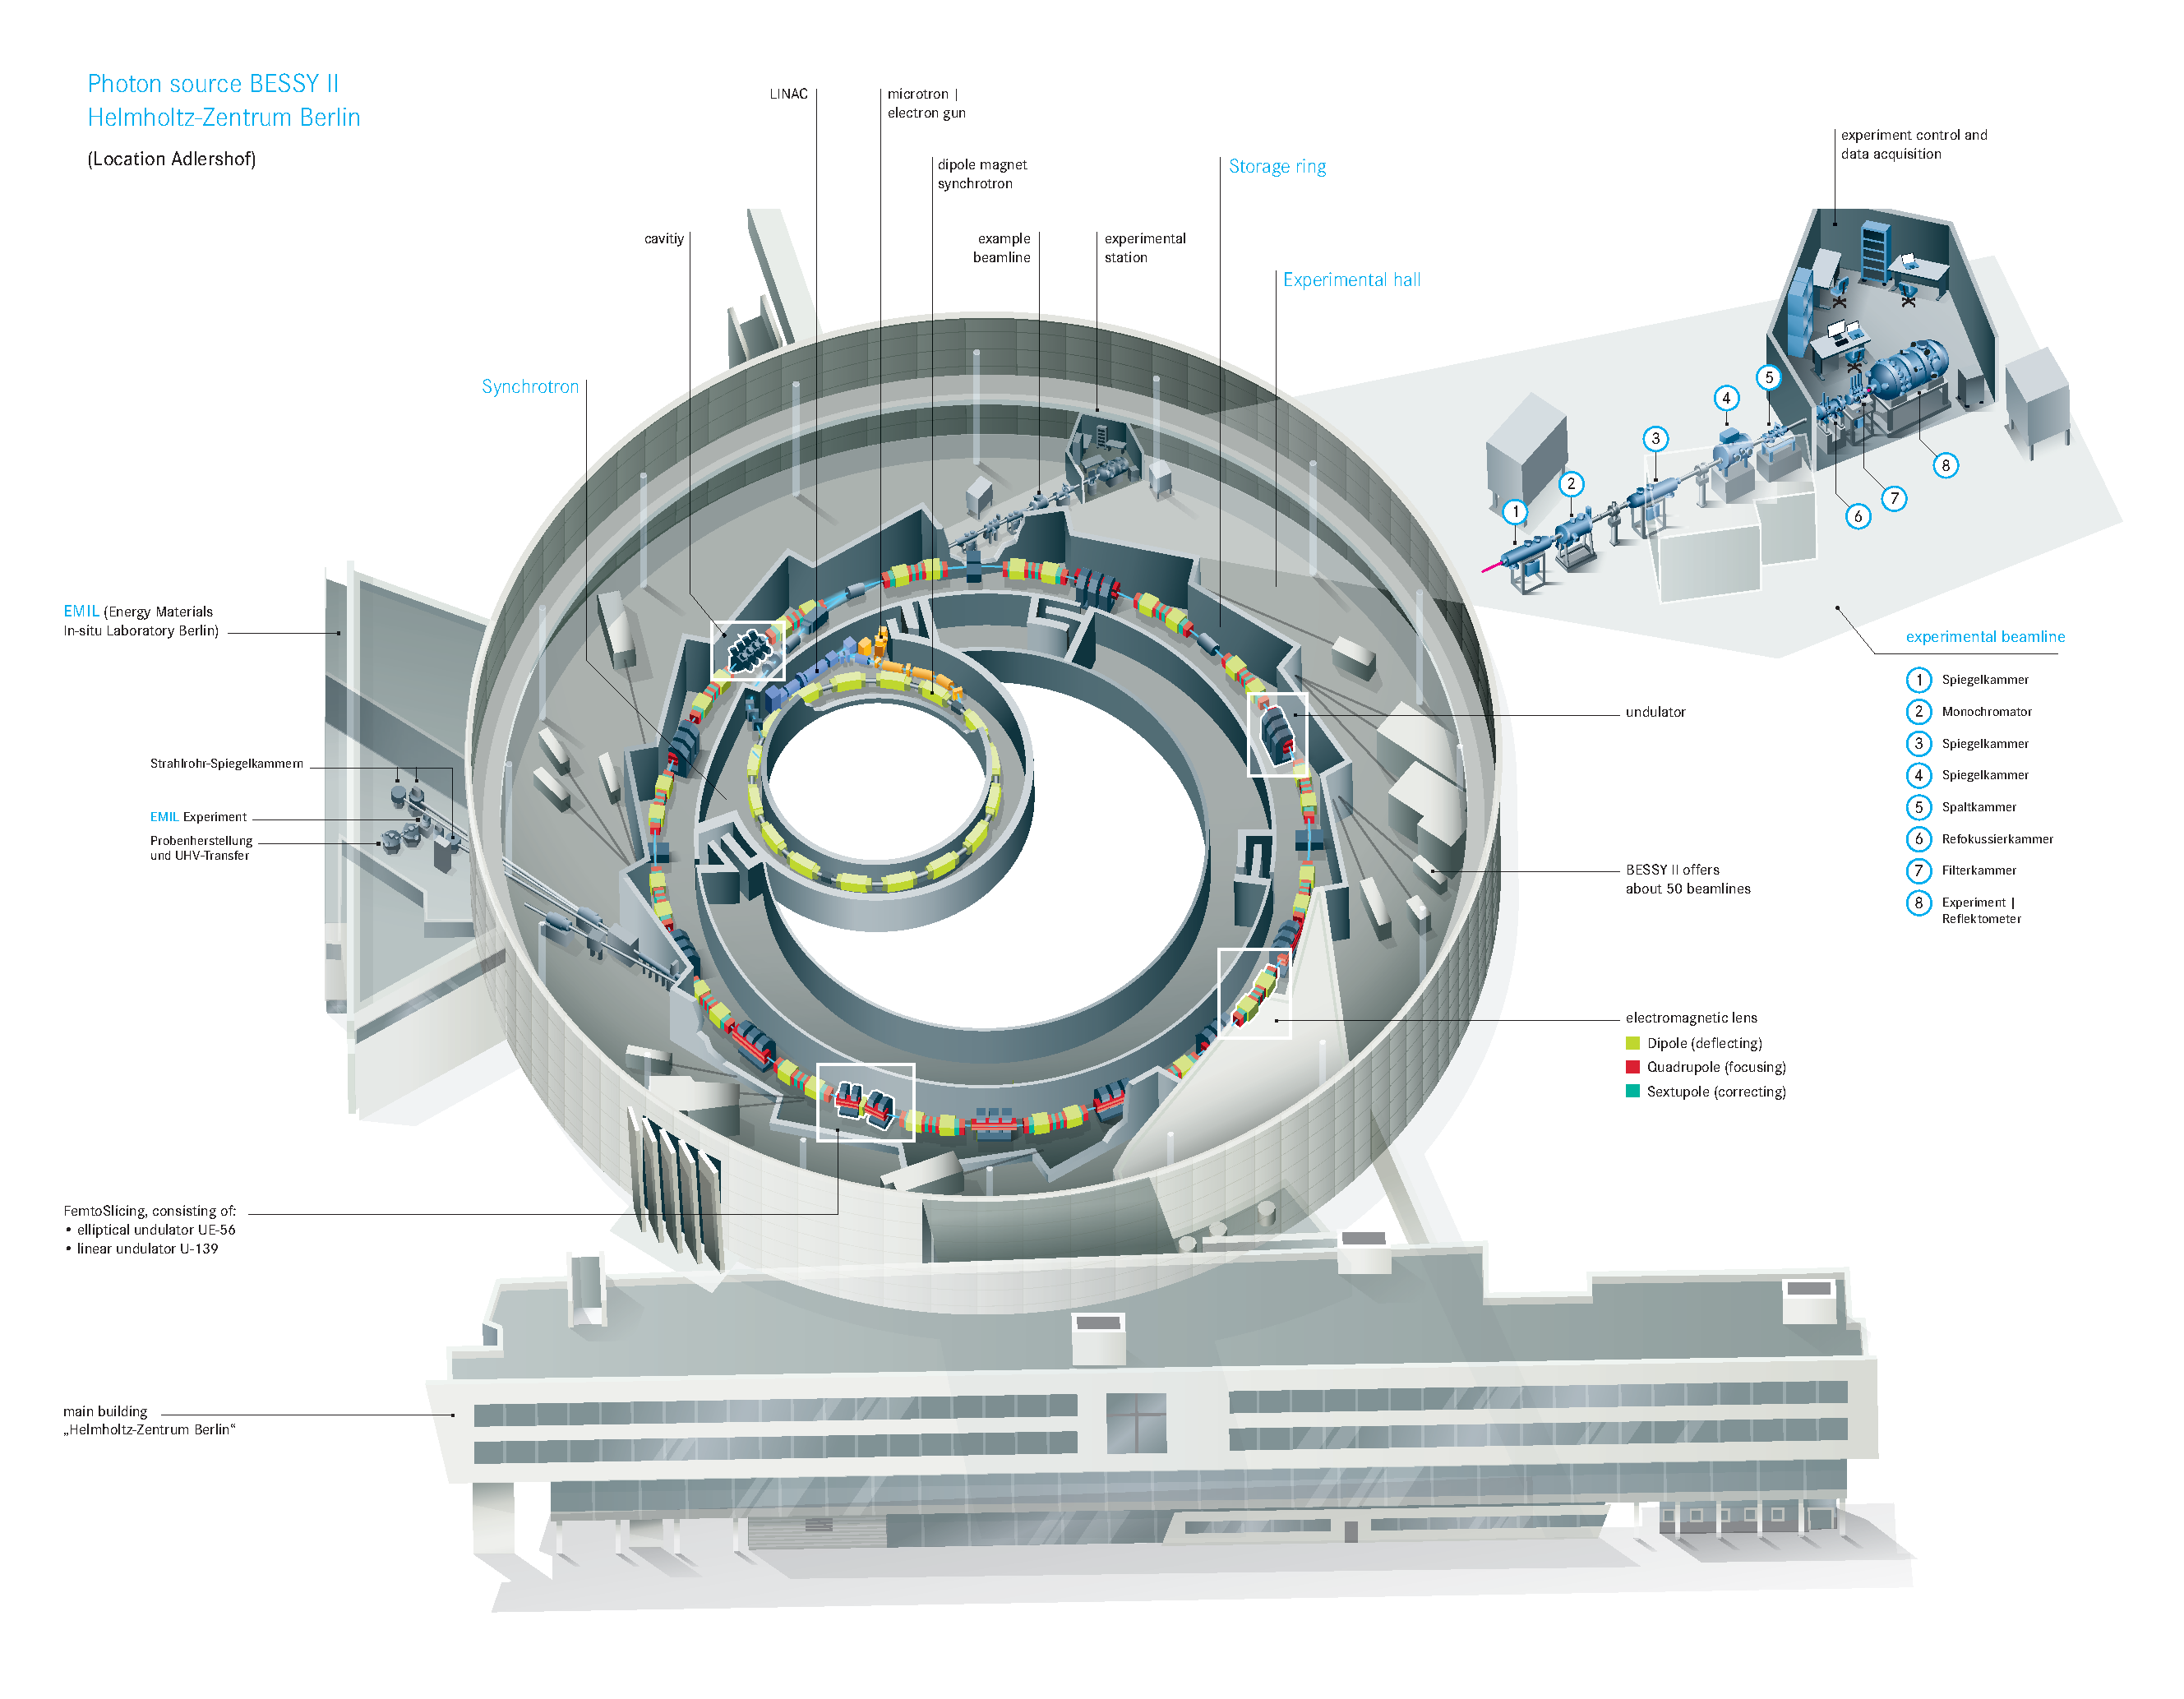
\includegraphics[width=0.8\textwidth,height=0.8\textheight,keepaspectratio]{img/bessy_acc_web.pdf}
    \caption[Bessy II facility]{\label{fig:bessy_acc_web} Bessy II facility (Source:~\cite{web:bessy_homepage})}
\end{sidewaysfigure}

In order to reach an energy of 1.7~GeV, the electrons undergo several chained accelerations (see \autoref{fig:bessy_acc_web}), namely:\todo{energies}
\begin{enumerate}
    \item an electron canon gives the electrons their first impulse
    \item a microtron accelerate them to an energy of XXX
    \item a LINAC (\textbf{lin}ear \textbf{ac}celerator) increase the energy to XXX
    \item the booster (a synchrotron) give them the final energy of XXX.
\end{enumerate}

When this energy is reached, the electrons are injected to the storage ring, which ensure that the electrons are kept at the same energy.

Because of the synchrotron radiation, the bunches of particles lose regularly their energy; therefore a new injections from the accelerations chain take place every XXX\todo{time} to repopulate the storage ring and stabilize its energy.

\section{Particle accelerator physics}
In order to understand the trajectory perturbations, the basic physics of the particle accelerator must be addressed.

\subsection{Synchrotron basics}
To study the beam trajectory, one possibility is to use the linear beam optics (by analogy between beam and light focusing and steering). We solely describe here what is needed in the next sections. A full reference can be found in~\cite{book:wille}. This section is mostly inspired by the chapter 3 of this same reference.

\subsubsection{Geometry -- Frame of reference -- Kinematics}
The term \emph{orbit} refers to the ideal trajectory of the particles, which is fixed by the construction of the accelerator.

The frame of reference is $K=(\vec{e}_x,\vec{e}_y, \vec{e}_s)$, which origin follows the beam. $\vec{e}_x$ is the horizontal axis directed towards the exterior of the orbit and normal to its curve, $\vec{e}_y$ is the vertical axis and $\vec{e}_s$ the tangential axis to the orbit.
\begin{figure}[!h]
    \centering
    \includegraphics[width=0.8\linewidth]{img/orbit_coordinates.pdf}
    \caption{\label{fig:coordinate system}Description of the co-moving coordinate system}
\end{figure}
Let $\varphi$ be the azimuth angle, oriented by $\vec{e}_y$. Then, since $ds = -R d\varphi$, we can write
\begin{equation}
\frac{d \varphi}{d t}  = -\frac{1}{R} \frac{d s}{d t}.
\end{equation}

Using the derivation formula of polar coordinate we can write:
\begin{align}
&\dot{\vec{e}}_x = \frac{d\vec{e}_x}{d t} = -\dot{\varphi} \vec{e}_s = \frac{1}{R} \dot{s}\vec{e}_s \nonumber \\
&\dot{\vec{e}}_y = 0 \\
&\dot{\vec{e}}_s = \frac{d\vec{e}_s}{d t} = \dot{\varphi} \vec{e}_x = -\frac{1}{R} \dot{s}\vec{e}_x \nonumber.
\end{align}

Let $\vec{r} = \vec{r}_0 + x\vec{e}_x + y \vec{e}_y$ be the position of a given particle in a Galilean reference frame (with $\vec{r}_0$ the position of the origin of the moving coordinates, see Fig.~\ref{fig:coordinate system}) and let's define $x'$ the spatial derivative with respect to $s$ so that:
\begin{equation}
\begin{aligned}
&\dot{x}= \frac{dx}{ds}\frac{ds}{dt} = x'\dot{s}  \\
&\ddot{x}= x''\dot{s}^2+x'\ddot{s}.
\end{aligned}
\end{equation}
It follows, after some algebraic manipulations:
\begin{align}
\label{eq:kinematics}
&\vec{r} = \vec{r}_0 + x\vec{e}_x + y \vec{e}_y \nonumber \\
&\dot{\vec{r}}= x' \dot{s} \vec{e}_x + y'\dot{s} \vec{e}_y  + \left(1+\frac{x}{R}\right)\dot{s}\vec{e}_s\\
&\ddot{\vec{r}}= \left[x'' \dot{s}^2 + x' \ddot{s} - \left( 1+\frac{x}{R} \right)\frac{\dot{s}^2}{R}\right] \vec{e}_x + (y''\dot{s}^2 + y'\ddot{s}) \vec{e}_y \nonumber \\
& \hspace{14em} + \left[\frac{2}{R}x'\dot{s}^2 +\left(1+\frac{x}{R}\right)\ddot{s}\right]\vec{e}_s \nonumber
\end{align}

\subsubsection{Hypotheses} We assume the following hypotheses are valid.
\begin{description}
    \item{H1 --} The particles move essentially parallel to $\vec{e}_s$: in the first order
    \begin{equation*}
        \vec{v} = v_s \vec{e}_s.
    \end{equation*}
    \item{H2 --} The magnetic field has only transverse components:
        \begin{equation*}
        \vec{B} = (B_x, B_y, 0)
        \end{equation*}
    \item{H3 --} The electric field is negligible with respect to the magnetic field.
    \item{H4 --} The velocity of the particle varies very slowly in a magnet: $\ddot{s} \approx 0$
    \item{H5 --} The particles move at relativistic velocities, so the effect of the magnetic field is negligible on longitudinal components: we consider only transverse components.
    \item{H6 --} The momentum of the particles is $p = p_0+\Delta p$, with the condition $\Delta p \ll p_0$ (which is well satisfied in accelerators).
\end{description}

\subsubsection{Equation of motion}
Newton's second law can be applied with the Lorentz force:
\begin{equation}
\dot{\vec{p}} = e(\vec{E}+\vec{v} \times \vec{B}) 
\end{equation}
which according to (H3) becomes
\begin{equation}
\ddot{\vec{r}} = \frac{e}{m}(\dot{\vec{r}} \times \vec{B})
\end{equation}

According to (H2), the magnetic field is only transversal, which yields:
\begin{equation}
\label{eq:lorentz_transv}
\ddot{\vec{r}} = \frac{e}{m}(\dot{\vec{r}} \times \vec{B})
= \frac{e}{m}
    \begin{pmatrix}
        -\left(1+\frac{x}{R}\right)\dot{s}B_y \\
        \left(1+\frac{x}{R}\right)\dot{s}B_x \\
        x'\dot{s}B_y - y'\dot{s}B_x
    \end{pmatrix}.
\end{equation}

Using (H5), we can focus on the x- and y-components, (H4) in Eq.~\eqref{eq:kinematics} allow us to remove every $\ddot{s}$ factors, so that Eq.~\eqref{eq:lorentz_transv} can be rewritten as
\begin{equation}
\begin{aligned}
x'' \dot{s}^2 - \left(1+\frac{x}{R}\right)\frac{\dot{s}^2}{R}
&= -\frac{e}{m} \left(1+\frac{x}{R}\right)\dot{s}B_y \\
y'' \dot{s}^2 &=    \left(1+\frac{x}{R}\right)\dot{s}B_x.
\end{aligned}
\end{equation}
Finally, because $p=mv$ and using Eq.~\eqref{eq:kinematics} combined with (H1), we can replace
\begin{equation}
m = \frac{p}{v} = \frac{p}{\scal{\vec{v}}{\vec{e}_s}} = \frac{p}{\left(1+\frac{x}{R}\right)\dot{s}}
\end{equation}
to obtain:
\begin{equation}
\begin{aligned}
x''-\left(1+\frac{x}{R}\right)\frac{1}{R} &= -\frac{e}{p} B_y\left(1+\frac{x}{R}\right)^2 \\
y'' &= \frac{e}{p} B_x\left(1+\frac{x}{R}\right)^2
\end{aligned}
\end{equation}

(H6) allow us to write, to first order:

\begin{equation*}
\frac{1}{p} = \frac{1}{p_0} \left(1-\frac{\Delta p}{p_0}\right).
\end{equation*}

Furthermore the magnetic field can be approximated to first order with:
\begin{equation}
\frac{e}{p_0} B_y = \frac{1}{R}-kx \qquad\qquad \frac{e}{p_0} B_x = -ky
\end{equation}
which yields
\begin{equation}
\begin{aligned}
x''-\left(1+\frac{x}{R}\right)\frac{1}{R} &= -\left(\frac{1}{R}-kx\right)\left(1-\frac{\Delta p}{p_0}\right)\left(1+\frac{x}{R}\right)^2 \\
y'' &= -ky\left(1-\frac{\Delta p}{p_0}\right)\left(1+\frac{x}{R}\right)^2
\end{aligned}
\end{equation}

Finally by removing terms of second order ($\frac{x}{R} \ll 1$, $\frac{\Delta p}{p_0} \ll 1$) we obtain the linear equations of motion in a magnetic structure:

\begin{empheq}[box=\fbox]{equation}
\begin{aligned}
x''(s) + \left(\frac{1}{R^2(s)} - k(s)\right) x(s) &= \frac{1}{R(s)}\frac{\Delta p}{p_0} \\
y''(s) + k(s) y(s) &= 0
\end{aligned}
\end{empheq}

\subsubsection{Beta function and betatron oscillation}
\subsubsection{Brightness and brilliance}
\label{sec:brightness_brillance}
(given by $\sigma'_{x,z}=\sqrt{\frac{\epsilon_{x,z}}{\beta_{x,z}}}$):
\begin{equation}
S = \frac{F}{2 \pi \sigma'_x \sigma'_z} = \frac{F \sqrt{\beta_x \beta_z}}{2 \pi \sqrt{\epsilon_x \epsilon_z}} = \frac{\text{photons}}{\text{s 0.1\% BW mrad$^2$ A}}
\end{equation}
while the brilliance relates to the transverse dimensions ($\sigma_{x,z}=\sqrt{\epsilon_{x,z}\beta_{x,z}}$):
\begin{equation}
B = \frac{F}{4 \pi^2 \sigma_x \sigma_z \sigma'_x \sigma'_z} = \frac{F}{4 \pi^2 \epsilon_x \epsilon_z} = \frac{\text{photons}}{\text{s 0.1\% mm$^2$ BW mrad$^2$ A}}
\end{equation}

These definitions vary in literature. These are taken from the K.~Wille book~\cite{book:wille}, and apply to Gaussian-shaped electron beams. The invariant idea is that both values are determinated by the beam emittance $\sigma$: the design of the accelerators and the correction are aimed at obtaining the smallest emittance $\sigma_{x,z}$ as possible.
\subsection{Booster and storage ring}
\todo[inline]{What is particular in storage ring}
Both the booster and the storage ring are synchrotrons. The former aims at accelerating the particles, whereas the latter aims at storing them with a constant energy. 

\section{Orbit and distortions}
\todo[inline]{Physics + examples = 1/2 - 1 pges}
\subsection{Theory}
The accelerators are designed so that the particles follow a given path, which is defined in the case of synchrotrons by the successive bendings involved by the magnets. As the precision of the positioning of the magnets is limited, some errors may destabilize the orbit and increase the dispersion of the particles around the theoretical orbit. In addition, the environment produces perturbations: for instance the 50~Hz of the main power, some not perfectly isolated magnetic sources.

In order not to lose electrons in the walls of the vacuum chamber but also to increase the brightness of the synchrotron radiations (and therefore to have focused electron beams), all these residual misalignment and magnetic field errors must be corrected.

\subsection{Distortions in BESSY II}



\chapter{Orbit correction}
\label{sec:correction}
\section{Some documented methods}
\todo[inline]{Best corrector, "...", inverse pb = 3 pages}
\section{State of the art at BESSY II}
\todo[inline]{2 pages}
\section{Acquisition of the transfer matrix}


% !TeX encoding = UTF-8
% !TeX spellcheck = en_US
% !TeX root = main.tex

\chapter{Localization of orbit perturbations}
\label{sec:localisation}

Correcting the orbit is costly and has never a perfect result. Instead of dealing with the effects, we can deal with the sources of the distortions. If none is really obvious (\textit{eg.} a non-isolated transformer, the 50~Hz perturbation of the main power), the orbit can give us some hints.

We call kick the place where the orbit brutally changes its angle as shown in \cref{fig:kick}.

\begin{figure}[!h]
	\centering
	\includegraphics[width=.9\linewidth]{img/kick}
	\caption{\label{fig:kick}Example of kick in the orbit}
\end{figure}

\section{Static perturbation}
\label{sec:loc_static}

\subsection{Theoretical setting of the problem}

Everything is described here with the phase variable 
\begin{equation}
\Psi = \int\limits_{0}^s \frac{d\sigma}{\beta(\sigma)}.
\end{equation}
The spatial variable is only used to have a connection between the result and the actual ring. The explanation will be led with the $x$ variable, but is also valid with the $y$ one.

Let one kick be at $\Psi = \hat{\Psi}$. The orbit is modified and oscillates with a constant period of $2 \pi$. Because there is {\em only one} kick and according to the closed orbit condition, the oscillation after the kick will be stable for one revolution. Furthermore, the orbit must be continuous on all points, thus at the kick position too.

Let's consider two revolutions, in order to be sure to find one full revolution without kick. Let $\Psi_\mathrm{ext} \in [0, 4 \pi Q]$ be this new phase (\textit{ext} for extended). The phase $\Psi_0$ where the kick happens is the one so that 
\begin{equation}
\exists (b, c) \in \mathbb{R}^2:
\forall \Psi \in [\Psi_0, \Psi_0 + 2 \pi Q], \quad
x(\Psi) = b \sin(\Psi + c)
\end{equation}

We have a problem with 3 unknowns to determine: $\Psi_0, b, c$. 

\subsection{Practical setting}

We have $m$ BPMs only, distributed around the orbit.
Therefore we define:
\begin{align}
\begin{cases}
\vec{\Psi} = [\Psi_0, \Psi_1, ..., \Psi_{m-1}] \\
\vec{x} = [x_0, x_1, ..., x_{m-1}]
\end{cases} \quad \mathrm{and} \quad
\begin{cases}
\vec{\Psi}_\mathrm{ext} = [\vec{\Psi}, \vec{\Psi}+2\pi Q ]\\
\vec{x}_\mathrm{ext} = [\vec{x}, \vec{x}]
\end{cases}
\end{align}

\subsection{Solving the problem}

The problem is solved in two steps: first the sine that fits at best the orbit is determined, and second the position of the kick verifying the closed orbit condition (or continuity condition) is found.

An algorithm is designed to find a sine over a revolution, beginning at each BPM and keep the one that fits at best:
\begin{align}
\forall k \in &[0, m-1], \nonumber \\
&\begin{cases}
\vec{\Psi}^k = [\vec{\Psi}_\mathrm{ext}(k), \vec{\Psi}_\mathrm{ext}(k+1), \cdots,  \vec{\Psi}_\mathrm{ext}(k+m-1)]\\
\vec{x}^k = [\vec{x}_\mathrm{ext}(k), \vec{x}_\mathrm{ext}(k+1), \cdots,  \vec{x}_\mathrm{ext}(k+m-1)]\\
\tilde{\vec{x}} = \mathtt{fit\_sine}(\vec{x}^k, \vec{\Psi}^k)
\end{cases}
\end{align}

It is then defined
\begin{equation}
k_0 = \underset{k \in [0, m-1]}{\textrm{argmin}}\{||\tilde{\vec{x}}-\vec{x}^k||_2\}
\end{equation}

If there where no noise in the signal, and if the precision over the phase $\Psi$ was infinite, then the kick would be exactly at $\Psi_{k_0}$. However in this case, it can only be said that the kick is around $\Psi_{k_0}$, and the closest sine is $\tilde{x}(\Psi) = b \sin(\Psi + c)$.

To find the exact position of the kick, the property of closed orbit is used: the orbit must be continuous also at the kick phase, which means that $\hat{\Psi}$ is the solution of
\begin{align}
b \sin(\Psi + c) &= b\sin(\Psi+c+2 \pi Q),\\
& \mathrm{with}~ \Psi \in [\Psi_{k_0}-A, \Psi_{k_0}+A] , A>0 \nonumber
\end{align}
or, with the numerical approach, 
\begin{equation}
\hat{\Psi} =  \underset{\Psi \in [\Psi_{k_0-A}, \Psi_{k_0+A}]}{\textrm{argmin}}\{|b \sin(\Psi + c) - b\sin(\Psi+c-2 \pi Q)|\}.
\end{equation}

$A$ was defined with the \textit{try-and-see} method and in the specific case of BESSY~II, $A=\frac{\pi}{4}$ suits.

\remark For this last step, we use a \textit{linspace} between $\Psi_{k_0}-A$ and $\Psi_{k_0}+A$ with more than 1000 points.

\subsection{Finding the good sine}
Several methods are possible to find the best matching sine, for example by using:
\begin{itemize}
	\item a pseudo-inversion
	\item a scalar-product with a sine (resp. a cosine)
\end{itemize}

\paragraph{Pseudo-inversion}
The problem can be set as a linear equation problem as follow.
\begin{align}
&\forall k \in [0,m-1], \tilde{x}(\Psi_k) = a_1 \sin(\Psi_k) + a_2 \cos(\Psi_k) + a \nonumber \\
%
\implies &
\begin{pmatrix}
1 & \sin(\Psi_0) & \cos(\Psi_0) \\
1 & \sin(\Psi_1) & \cos(\Psi_1) \\
\vdots & \vdots & \vdots \\
1 & \sin(\Psi_{m-1}) & \cos(\Psi_{m-1}) \\
\end{pmatrix}
\begin{pmatrix}
a \\ a_1 \\ a_2
\end{pmatrix}
=
\begin{pmatrix}
x_0 \\ x_2 \\ \vdots \\ x_{m-1}
\end{pmatrix} \nonumber
\\
%
\implies &
\begin{pmatrix}
a \\ a_1 \\ a_2
\end{pmatrix}
= 
\mathrm{pseudo\_inv}
\begin{pmatrix}
1 & \sin(\Psi_0) & \cos(\Psi_0) \\
1 & \sin(\Psi_1) & \cos(\Psi_1) \\
\vdots & \vdots & \vdots \\
1 & \sin(\Psi_{m-1}) & \cos(\Psi_{m-1}) \\
\end{pmatrix}
\begin{pmatrix}
x_0 \\ x_2 \\ \vdots \\ x_{m-1}
\end{pmatrix}
\end{align}

The pseudo inverse is calculated in \texttt{Matlab} with 
\begin{verbatim}
        a = M\x
\end{verbatim}
and in \texttt{python} with the least-squares method
\begin{verbatim}
        a = numpy.linalg.lstsq(M, x).
\end{verbatim}

\paragraph{Scalar product with a sine (resp. cosine)}
Since the orbit is expected to be written as
\begin{equation*}
x(\Psi) = a+ a_1 \sin(\Psi) + a_2 \cos(\Psi)
\end{equation*}
it can also be described as
\begin{equation}
x(\Psi) = \scal{x}{1} + \scal{x}{\sin} \sin(\Psi) + \scal{x}{\cos} \cos(\Psi)
\end{equation}
with $\scal{f}{g}$ being the scalar product for real functions: $\int_T f(t)g(u)dt$.

In the numerical case, the scalar product is approximated by its vectorial counterpart by

\begin{align*}
\scal{\vec{f}}{\vec{g}}: \quad
 &\mathcal{R}^n \times \mathcal{R}^n \longrightarrow \mathcal{R} \\
 & (\vec{f},\vec{g}) \quad\longmapsto \quad \frac{1}{n}\sum\limits_{k=0}^{n-1} f_i g_i
\end{align*}

\paragraph{Coefficient format}
By defining $b = \sqrt{a_1^2+a_2^2}$ and $c = \mathrm{atan2}(a_2, a_1)$ the previous formulas can be written
\begin{equation*}
\tilde{x}(\Psi) = a + a_1 \sin(\Psi) + a_2 \cos(\Psi) = a + b \sin(\Psi + c).
\end{equation*} 

\section{Harmonic perturbations}
In this section, we deal with a perturbation at a given frequency $f$. The training data is the time signal of all BPMs.

As the perturbation has a known frequency, its complex amplitude can be extracted from the signal of each BPM with a Fourier transform:

\begin{equation}
\forall i \in [1, \mathrm{BPM\_nb}], \qquad 
\begin{cases}
\vec{X}_i = \mathrm{FFT}(\vec{x}_i) \\
c_i = \vec{X}_i(f)
\end{cases}
\end{equation}

\subsection{Case of a unique perturbation source}

If the perturbation is unique, then all complex amplitude exactly describe the same sine of frequency $f$ and phase $\alpha_0$. The complex vector $\vec{c}$ can thus be fully described with $\vec{\hat{c}}$, which is real.

\begin{align}
&\alpha_0 = \underset{\alpha \in [0, 2\pi]}{\textrm{argmin}}\{\mathcal{R}e (\vec{c} \cdot e^{-j\alpha}) \} \label{eq:harm_perturb_opt}\\
&\vec{\hat{c}} = \mathcal{I}m (\vec{c} \cdot e^{-j\alpha_0})
\end{align}

The new signal $\vec{\hat{c}}$ can be used as an orbit signal: each BPM have one orbit amplitude. The kick can be extracted from it with the previous method described in \cref{sec:loc_static}.

\remark To achieve the phase optimization given in \cref{eq:harm_perturb_opt}, the Karhunen–Loève transform (or principal component analysis) can be used~\cite{book:wang_2012}. A description of the algorithm is given in \cref{apx:KLT}. If the results are exactly the same, this allows the problem to be solved within a broader theoretical setting. The goal is not anymore to see the cosine part vanish but to deal with the perturbation space in which the distortion is the largest. In theory, dealing with each principal component would allow to find the position of each perturbation source.

\subsection{Case of several perturbation sources}
If there are several perturbation sources, a $\alpha_0$ that let the cosine part vanish cannot be found. 


\section{Implementation}
\begin{python}[caption=Get the kick]
	import matplotlib.plt as plt
	import search_kick.core as skcore
	
	# Dataset
	orbit = ..
	phase = ..
	tune = ..
	
	# Get the kick and rebuild the ideal sine
	kick_phase, sin_coef = skcore.get_kick(orbit, phase, tune)
	sine, phase_th = skcore.build_sine(kick_phase, tune, sin_coef)
	
	# Plot the results
	plt.plot(phase, orbit, '-b')
	plt.plot(phase_th, sine, '-g')
	plt.axvline(kick, -2, 2)	
\end{python}


\section{Examples}


\chapter{Harmonic perturbations}
\label{sec:harmonic_distorsion}
\section{Data analysis}

\section{Correction}
\section{Example: the 10 Hz perturbation}

\begin{python}[caption={Perturbation localisation, f = 10 Hz}]
	import matplotlib.plt as plt
	import search_kick.core as skcore
	import search_kick.tools as sktools
	
	# Dataset
	phase = ...
	tune = ...
	time_signal = ....  # nb_bpms lines, nb_samples colunms
	fs = 500  # sampling rate (Hz)
	
	f = 10  # frequency to extract (Hz)
	
	# Extract cosine and sine amplitude with a FFT transform
	a, b = skcore.extract_cos_sin_withfft(values, fs, f)
	
	# Optimize to only have the sine amplitude
	step_size = 0.1
	a_opt, b_opt, alpha_0 = sktools.maths.optimize_rotation(a, b, step_size)
	
	# Get the kick
	kick, sin_coef = skcore.get_kick(a_opt, phase, tune)
	sine, phase_th = skcore.build_sine(kick_phase, tune, sin_coef)
	
	# Plot the results
	plt.plot(phase, a_opt, '-b')
	plt.plot(phase, b_opt, '-m')  # cosine amplitudes: to be sure that it was a unique perturbation
	plt.plot(phase_th, sine, '-g')
	plt.axvline(kick, -2, 2)
	
\end{python}

KLT~\cite{book:wang_2012}
%%
%  Bibliography
%%
\bibliographystyle{IEEEtran}
\bibliography{biblio.bib}

\end{document}

